\subsection{$K^-pp$ assumption}
Finally, we assume that the unknown excess is fully attributed to the $K^-pp$ formation, and evaluate its differential cross section at $\theta_{lab}=0^\circ$. %in the bound region. %The integrated cross section in the bound region is evaluated for the assumed decay modes in the following.
\subsubsection{CDS tagging efficiency and the signal killing ratio by the $\Sigma^\pm$-decays removal}
To evaluate the reaction cross section from the number of excess in Fig. \ref{fig-nbg}, we need to assume the decay modes of the $K^-pp$ and evaluate the CDS tagging efficiencies ($A_{CDS}$)  for each decay mode. The signal survival ratios after the removal of the neutrons from the $\Sigma$ decays ($\epsilon_{\rm \Sigma\ cut}$) should be also evaluated, since the excess is integrated in the spectrum after the removal of the  $\Sigma$-decay events. They are evaluated with the simulation by changing the $K^-pp$ binding energy. The $K^-pp$ is assumed to decay isotropically with following decay modes: 
\begin{eqnarray}
K^-pp&\to& (\pi\Sigma)^0 p  \label{decay-pisp}\\
 &\to& \Lambda p  \label{decay-lp}\\
&\to& \Sigma^0 p. \label{decay-sp}
\end{eqnarray}
Reaction (\ref{decay-pisp}) is naturally expected from the decay mode of $\Lambda(1405)$ and it is expected to be dominant if the binding energy is small. However, this branch would be forbidden if the binding energy is larger than 100.53 MeV. Reaction (\ref{decay-lp}) is the decay channel FINUDA and DISTO observed as the ``$K^-pp$" candidates. Reaction (\ref{decay-sp}) has the same decay products with reaction (\ref{decay-lp}) except for a $\gamma$ emitted in $\Sigma^0\to \Lambda\gamma$.

The obtained values of $A_{CDS}$ and $\epsilon_{\rm \Sigma\ cut}$ are shown in Fig. \ref{fig-kppcdstag}. 


\begin{figure}[]
\begin{center}
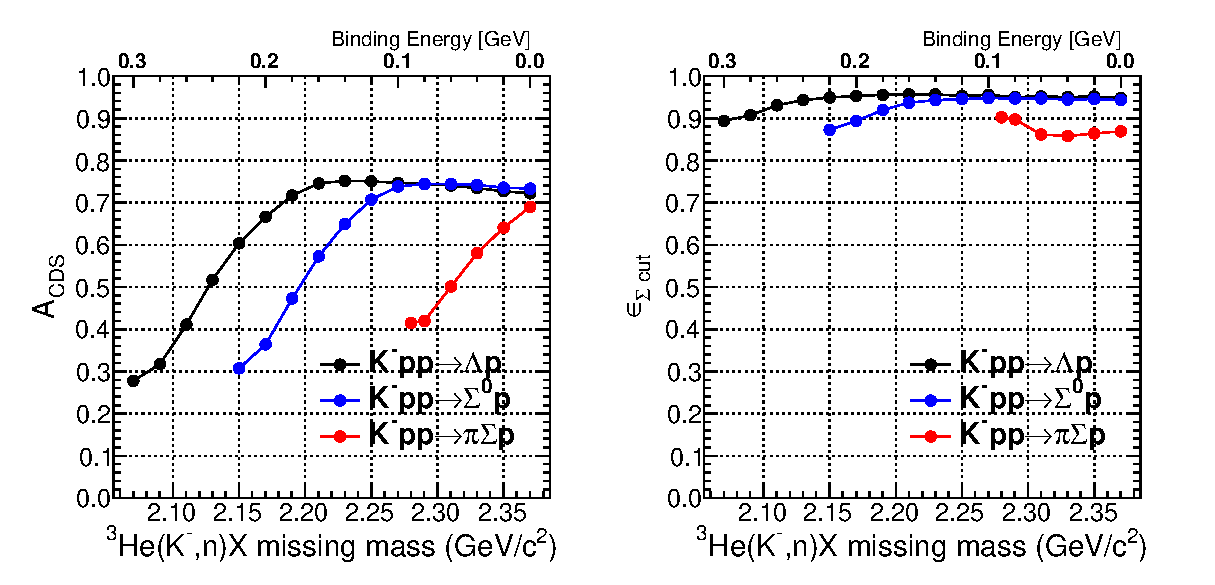
\includegraphics[width=\columnwidth]{./fig/kpp-cdstag.eps}
\caption[Simulated CDS tagging efficiencies and signal survival rates in the $\Sigma$-decays cut.]{(left) Simulated CDS tagging efficiencies and (right) signal survival rates in the $\Sigma$-decays cut for each decay mode.}
\label{fig-kppcdstag}	
\end{center}
\end{figure}  

\subsubsection{Differential cross section under the $K^-pp$ assumption}
We evaluate the differential cross section at $\theta_{lab}=0^\circ$ assuming the excess is fully attributed to the $K^-pp$ formation. The cross sections for each decay mode are obtained to be:
\begin{eqnarray*}
1.21 \pm 0.05 (stat.) \pm 0.21 (syst.)\  {\rm mb/sr} & & (K^-pp \to \Lambda p) \\
1.22 \pm 0.05 (stat.) \pm 0.21 (syst.)\  {\rm mb/sr} & & (K^-pp \to \Sigma^0 p) \\
1.56 \pm 0.06 (stat.) \pm 0.27 (syst.)\  {\rm mb/sr} & & (K^-pp \to \pi\Sigma p) 
\end{eqnarray*}
the systematic error is estimated as the quadratic sum of two kinds of errors: One is the systematic error of the excess yield summarized in Table \ref{tab-bound}, and the other is $\sim$ 17\% relative uncertainty of the normalization factor summarized in Table \ref{tab-ncs}.
\\

The derived differential cross section of the excess under the $K^-pp$ assumption is similar to that of the theoretical calculation by Koike and Harada\cite{Koike:2009cx}. They predicted the cross section is of the order of mb/sr integrated in the bound region. 

In terms of the spectral shape of the excess, a direct comparison is impossible since the experimental spectrum is obtained under the semi-inclusive condition. However, the tagging efficiencies of the CDS shown in Fig. \ref{fig-kppcdstag} have similar tendencies to the phase space suppression factor used in the derivation of the theoretical spectrum. Thus the peak structure in Fig. \ref{fig-koike}(d) or the cusp in Fig. \ref{fig-koike}(c) would be further enhanced in our semi-inclusive spectrum while the spectra in Fig.\ref{fig-koike}(a)(b) would not change drastically.

As a consequence, the case of Fig. \ref{fig-koike}(a) is most similar to our experimental spectrum. It means that our experimental data favors a shallow binding energies of B.E. $<$40 MeV with moderately large width of $\Gamma$=50$\sim$100 MeV for the $K^-pp$ state, if the $K^-pp$ assumption is the case. These binding energy and width are consistent with most of the few body calculations listed in Table \ref{tab-kppsummary}. 

\section{Upper limit for the formation cross section of deeply-bound $K^-pp$ state\label{sec-upper}}
In the previous section, we evaluated the differential cross-section of the excess, by assuming that the excess is fully attributed to the $K^-pp$, in the missing-mass region from 2.29 to 2.37 GeV/$c^2$ corresponding to the binding energy from 0 to 80 MeV. In the deep bound region below 2.29 GeV/$c^2$ corresponding to the binding energy of larger than 80 MeV, we can assume the smooth background as already discussed. Therefore, we evaluate the upper limit for the formation of a possible peak structure in this section. Such a peak, if existed, would be a dibaryon state with strangeness -1. Although it may not be the $K^-pp$, [$\bar K \otimes\{NN\}_{I=1}]_{I=1/2}$ state, here we assume the dibaryon state as the $K^-pp$ decaying into $\Lambda p$ to determine the upper limit.

\subsection{Spectral fitting} 
\subsubsection{$K^-pp$ shape}
The Breit-Wigner distribution is employed as the intrinsic shape of the $K^-pp$. However, in the semi-inclusive spectrum, the shape should be distorted by the charged-particle tagging in the CDS and the $\Sigma$-decays removal, which depend on its binding energy as shown in Fig. \ref{fig-kppcdstag}. The decay mode assumed here is $K^-pp\to \Lambda p$ only. In addition, the shape is smeared by the resolution of the detector system $\sigma_{MM}$. This resolution also depends on the binding energy as shown in Fig. \ref{fig-mmresol}. Then the peak distribution $F(x; M_S, \Gamma)$ is given by,
\begin{eqnarray*}
F(x; M_S, \Gamma)&=& \int f(\tau)*g(x-\tau,\sigma_{MM}(\tau))d\tau \\
f(x; M_S, \Gamma) &=&  \frac{d\sigma}{d\Omega}(\theta_{lab}=0)\cdot\left(\frac{1}{2\pi}\frac{\Gamma}{(x-M_s)^2+\Gamma^2/4}\right) \cdot A_{cds}(x) \cdot \epsilon_{\Sigma\rm{cut}}(x)\\
g(x;\sigma) &=& \frac{1}{\sqrt{2\pi}\sigma}\exp\left(-\frac{x^2}{2\sigma^2}\right),
\end{eqnarray*}
where $M_S$ and $\Gamma$ are the mass and the width of the $K^-pp$ state, respectively. 
As the background, a second order polynomial function is employed.
\subsubsection{Fitting}
The $\Sigma$-decay subtracted spectrum is fitted with the above $K^-pp$ distribution and the background in the missing-mass region from 1.50 GeV/$c^2$ to 2.29 GeV/$c^2$. The fitting parameters are the differential cross section $\frac{d\sigma}{d\Omega}(\theta_{lab}=0^\circ$) of the $K^-pp$ and the background function. %We accepted the reduce $\chi^2$ value less than 1.5.
\subsubsection{Derivation of the upper limit from the fitting result}
To evaluate the upper limit of the cross section, we adopt a Baysian approach; we renormalize the probability distribution functions by eliminating an unphysical region corresponding to $d\sigma/d\Omega<0$. The error of the cross section is evaluated by adding the statistical error obtained by the fitting and the systematic error of 17\% obtained in Sec. \ref{sec-norm}, quadratically. Then the upper limit at 95\% confidence level is calculated with the cross section and the evaluated error.

\subsection{Result and comparison with other $K^-pp$ studies}
The spectral fittings are performed with the $K^-pp$ widths of 20, 60, 100 MeV/$c^2$ and the mass from 2.1 to 2.28 GeV/$c^2$ in increments of 20 MeV/$c^2$. The resultant upper limits a 95\% confidence level are 0.02$\sim$0.4 mb/sr as shown in Fig. \ref{fig-upper}. 

\begin{figure}[]
\begin{center}
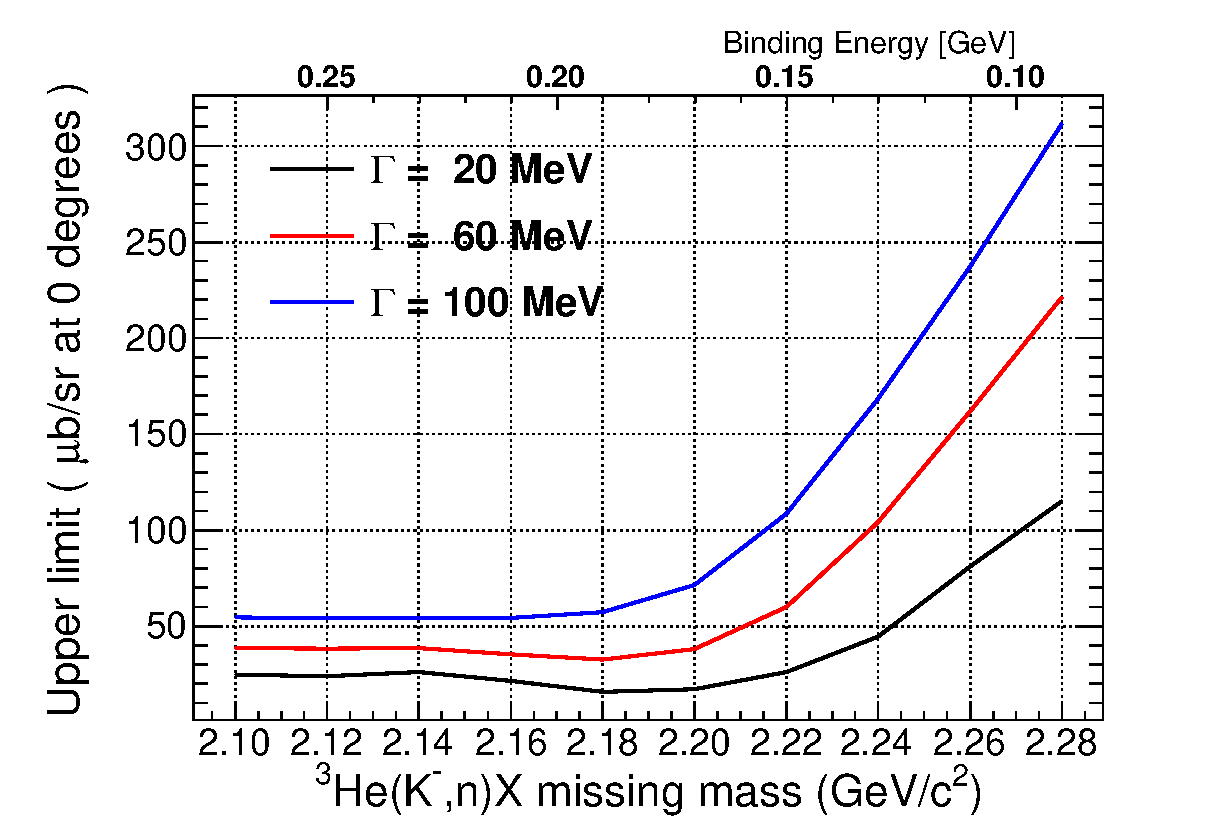
\includegraphics[width=12cm]{./fig/mm-upper.eps}
\caption[Upper limits of the formation cross section for a strange dibaryon state.]{Upper limits of the formation cross section at $\theta_{lab}=0^\circ$ and a 95\% confidence level for a strange dibaryon state decaying into $\Lambda p$ final state.}
\label{fig-upper}
\end{center}
\end{figure}  

Now we compare the obtained results with possible candidates of the deeply-bound $K^-pp$ states reported by FINUDA\cite{PhysRevLett.94.212303} and DISTO\cite{Yamazaki:2010ef} groups. They claimed the observation of the $K^-pp$ state with (binding-energy, width)=(115, 67) MeV and (105, 118) MeV in $\Lambda p$ final state, respectively. We have found no statistically significant structure in those region, and the upper limits of the formation cross section via $\Lambda p$ decay mode have been obtained to be $\sim$ 0.25 mb/sr and $\sim$ 0.35 mb/sr for the $K^-pp$ states FINUDA and DISTO claimed, respectively. The results also contradict the theoretical calculation by Koike and Harada\cite{Koike:2009cx}, where potentials obtained from the results of FINUDA and DISTO make a distinct peak structure in the $^3$He($K^-,n)X$ missing-mass spectrum at $\theta=0^\circ$, with more than 1 mb/sr cross section in the bound region as shown in Fig. \ref{fig-koike}(d).